% System diagram of the final paper: the v5 flow (whiteboard "Flujo RAG de la v5"), redrawn in English. TikZ; compile with pdflatex.
\documentclass[tikz,border=3pt]{standalone}
\usepackage[T1]{fontenc}
\usepackage[scaled=0.92]{helvet}
\renewcommand{\familydefault}{\sfdefault}
\usetikzlibrary{arrows.meta,calc,shapes.geometric,shapes.symbols,shapes.misc}
\definecolor{ragfill}{HTML}{DCEEFB}\definecolor{ragline}{HTML}{0072B2}
\definecolor{wfill}{HTML}{FFFFFF}\definecolor{wline}{HTML}{4D4D4D}
\definecolor{orfill}{HTML}{E3F4EC}\definecolor{orline}{HTML}{009E73}
\definecolor{outfill}{HTML}{FFF2CC}\definecolor{outline}{HTML}{B07D00}
\definecolor{zone}{HTML}{9A9A9A}
\hyphenpenalty=10000\exhyphenpenalty=10000
\begin{document}
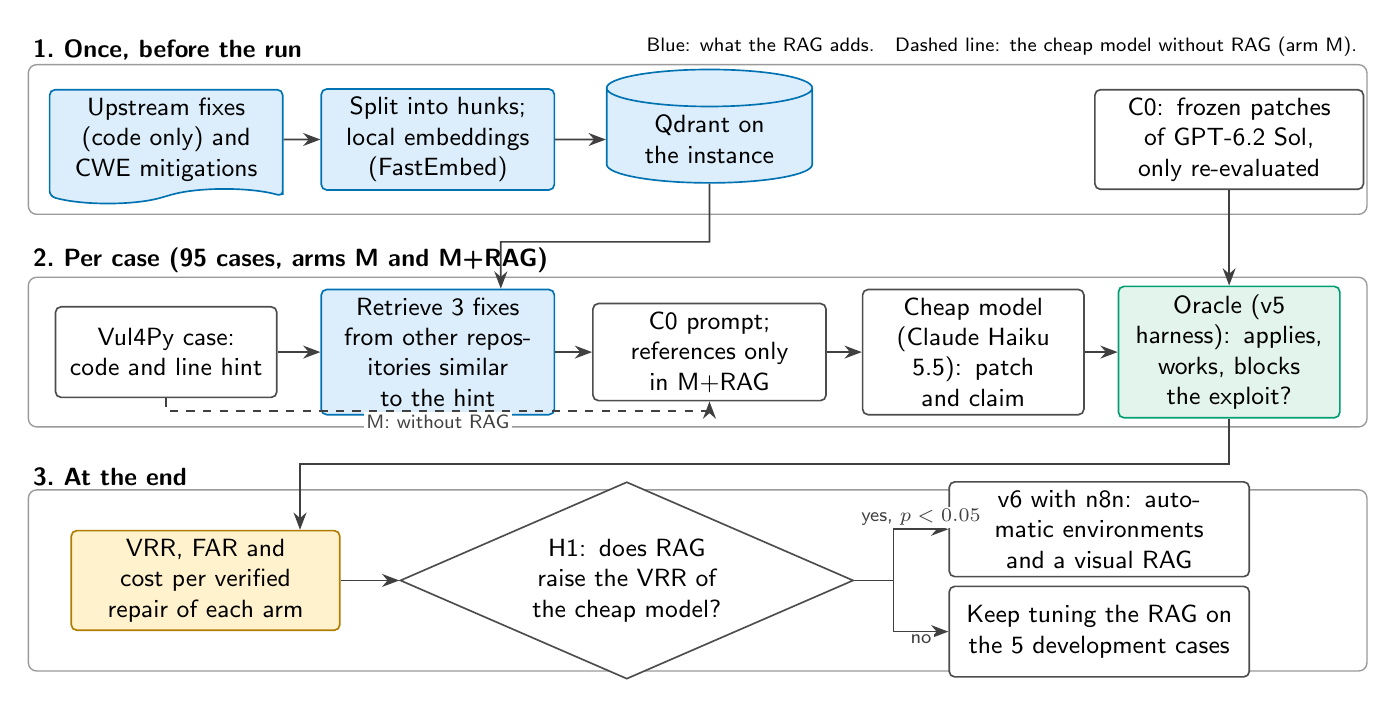
\begin{tikzpicture}[
  font=\small,
  box/.style={draw, rounded corners=2pt, align=center, text width=#1, minimum height=1.15cm, inner sep=3pt, line width=0.6pt},
  box/.default=2.75cm,
  rag/.style={fill=ragfill, draw=ragline},
  plain/.style={fill=wfill, draw=wline},
  arr/.style={-{Stealth[length=2.2mm]}, line width=0.6pt, color=black!75},
  lab/.style={font=\scriptsize, fill=white, inner sep=1pt},
  bandtitle/.style={font=\small\bfseries, anchor=south west, inner sep=1.5pt}
]
% ---------------------------------------------------------------- bands
\foreach \yt/\yb/\t in {0.95/-0.95/{1.\ Once, before the run}, -1.75/-3.65/{2.\ Per case (95 cases, arms M and M+RAG)}, -4.45/-6.75/{3.\ At the end}}{
  \draw[zone, rounded corners=3pt, line width=0.5pt] (0,\yb) rectangle (17.0,\yt);
  \node[bandtitle] at (0,\yt) {\t};
}
% ---------------------------------------------------------------- band 1
\node[box, rag, shape=tape, tape bend top=none, minimum height=1.1cm] (corpus) at (1.75,0)
  {Upstream fixes (code only) and CWE mitigations};
\node[box, rag] (embed) at (5.2,0) {Split into hunks; local embeddings (FastEmbed)};
\node[box=2.4cm, rag, cylinder, shape border rotate=90, aspect=0.18, minimum height=1.3cm, rounded corners=0pt] (qdrant) at (8.65,0)
  {Qdrant on the instance};
\node[box=3.2cm, plain] (c0) at (15.25,0) {C0: frozen patches of GPT-6.2 Sol, only re-evaluated};
% ---------------------------------------------------------------- band 2
\node[box=2.6cm, plain] (case) at (1.75,-2.7) {Vul4Py case: code and line hint};
\node[box, rag] (retr) at (5.2,-2.7) {Retrieve 3 fixes from other repositories similar to the hint};
\node[box, plain] (prompt) at (8.65,-2.7) {C0 prompt; references only in M+RAG};
\node[box=2.6cm, plain] (llm) at (12.0,-2.7) {Cheap model (Claude Haiku 5.5): patch and claim};
\node[box=2.6cm, fill=orfill, draw=orline] (oracle) at (15.25,-2.7) {Oracle (v5 harness): applies, works, blocks the exploit?};
% ---------------------------------------------------------------- band 3
\node[box=3.2cm, fill=outfill, draw=outline] (metrics) at (2.25,-5.6) {VRR, FAR and cost per verified repair of each arm};
\node[draw, diamond, aspect=2.3, align=center, text width=3.1cm, inner sep=1pt, line width=0.6pt, fill=wfill, draw=wline] (h1) at (7.6,-5.6)
  {H1: does RAG raise the VRR of the cheap model?};
\node[box=3.6cm, plain] (v6) at (13.6,-4.95) {v6 with n8n: automatic environments and a visual RAG};
\node[box=3.6cm, plain] (tune) at (13.6,-6.25) {Keep tuning the RAG on the 5 development cases};
% ---------------------------------------------------------------- arrows
\draw[arr] (corpus) -- (embed);
\draw[arr] (embed) -- (qdrant);
\draw[arr] (qdrant.south) -- (8.65,-1.3) -- (6.0,-1.3) -- ($(retr.north)+(0.8,0)$);
\draw[arr] (case) -- (retr);
\draw[arr] (retr) -- (prompt);
\draw[arr] (prompt) -- (llm);
\draw[arr] (llm) -- (oracle);
\draw[arr, dashed] (case.south) -- (1.75,-3.45) -| node[lab, pos=0.25, below] {M: without RAG} (prompt.south);
\draw[arr] (c0) -- (oracle);
\draw[arr] (oracle.south) -- (15.25,-4.12) -- (3.45,-4.12) -- ($(metrics.north)+(1.2,0)$);
\draw[arr] (metrics) -- (h1);
\draw[arr] (h1.east) -- ++(0.5,0) |- node[lab, pos=0.75, above] {yes, $p<0.05$} (v6.west);
\draw[arr] (h1.east) -- ++(0.5,0) |- node[lab, pos=0.75, below] {no} (tune.west);
% ---------------------------------------------------------------- legend
\node[font=\scriptsize, anchor=east, align=right] at (17.0,1.18) {Blue: what the RAG adds.\quad Dashed line: the cheap model without RAG (arm M).};
\end{tikzpicture}
\end{document}
